This chapter discusses the all the aspects related to the main JFFS3 entity~--
the tree. Please, refer to section \ref{ref_SectionIndexing} for basic
information about the JFFS3 tree.

%
% OBJECTS
%
\subsection{Objects} \label{ref_SectionObjects}

JFFS3 keeps file system objects in the leaf level of the tree (in leaf nodes)
and the following is the list of supported objects.

\begin{enumerate}

\item \emph{Data} objects contain files' data and are kept in \emph{data
nodes}. Each data node holds one \mbox{RAM page} bytes of data (i.e.,
\texttt{PAGE\_SIZE} which is 4K on most \mbox{32-bit} architectures). But of
course, in case of small files (less then one RAM page bytes) and files'
tails~-- less data data may be put to the data node.

%
% Figure with an data objects illustration
%
\begin{figure}[h]
\begin{center}
\begin{htmlonly}
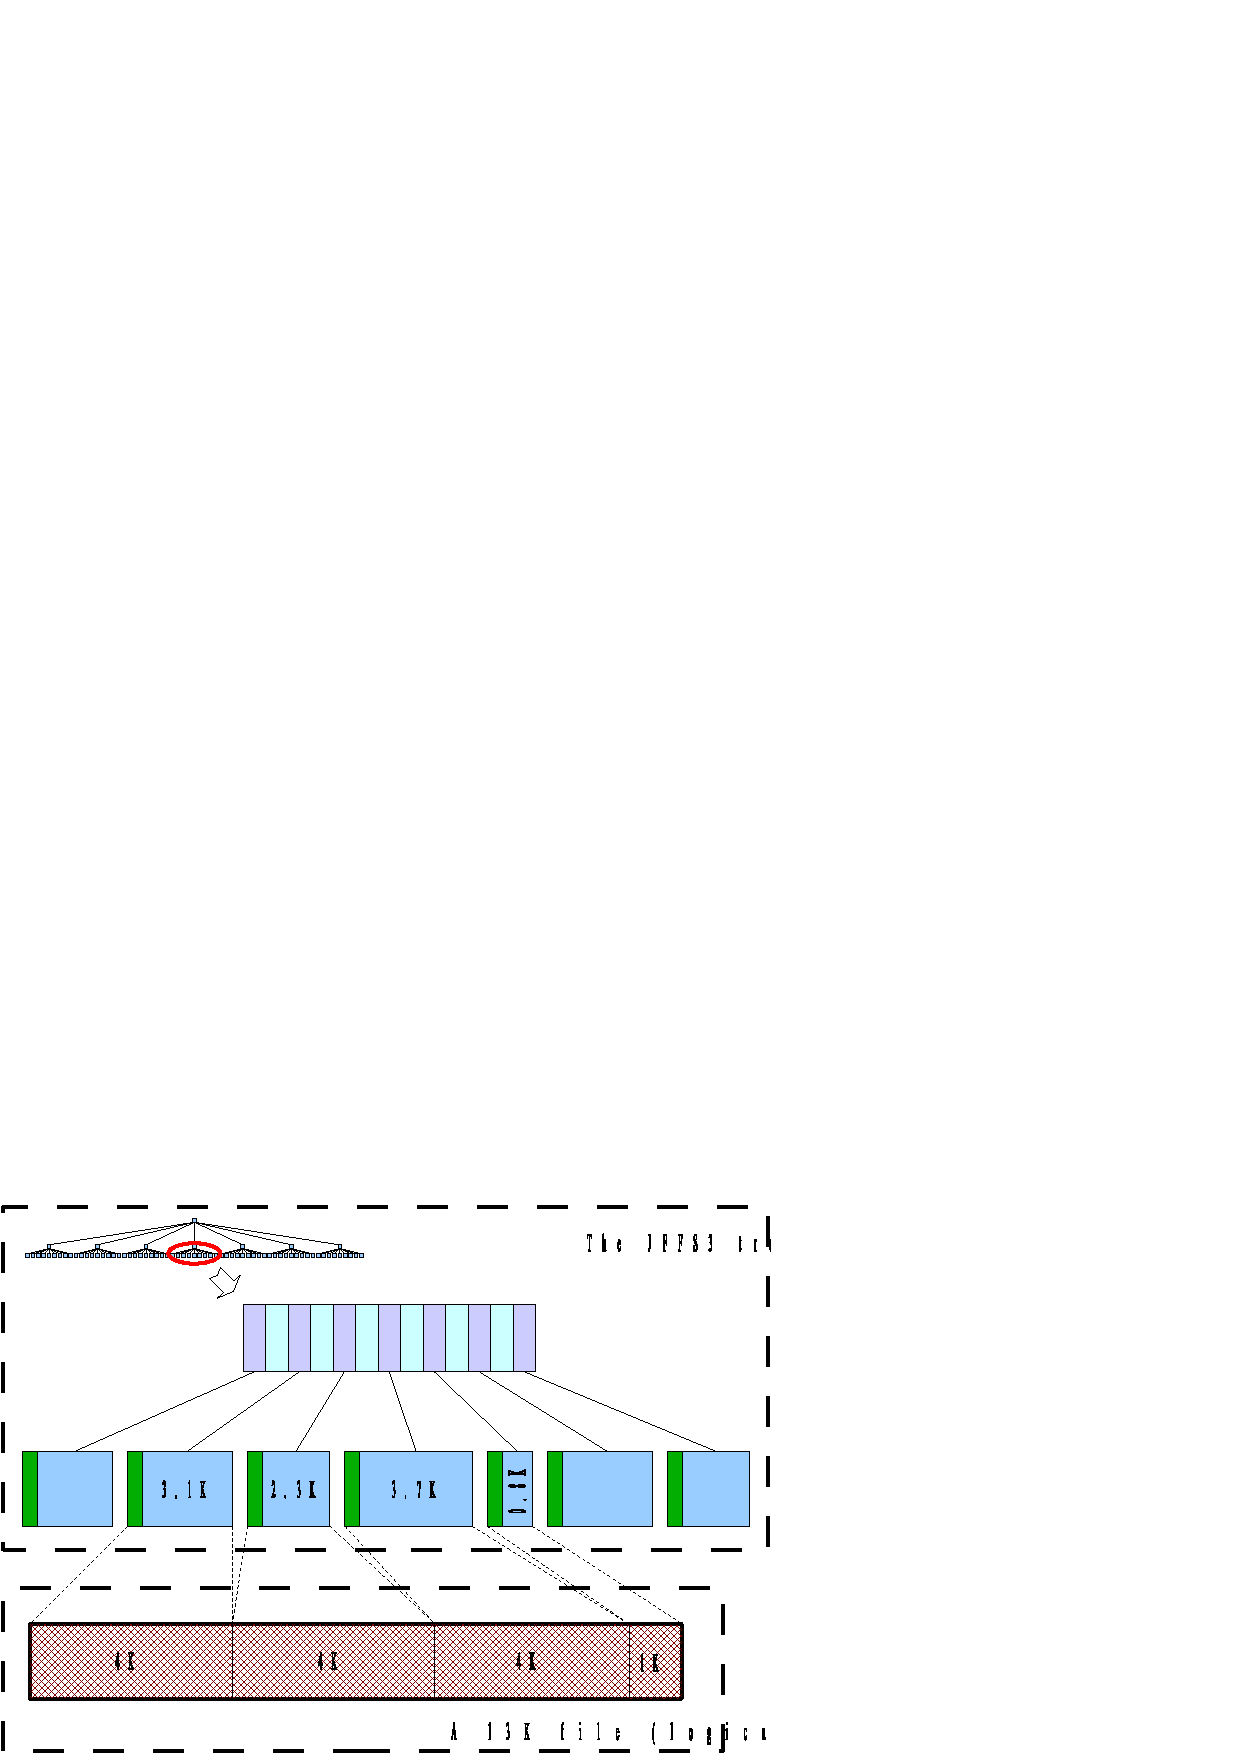
\includegraphics{pics/dataobj-01.png}
\end{htmlonly}
%begin{latexonly}
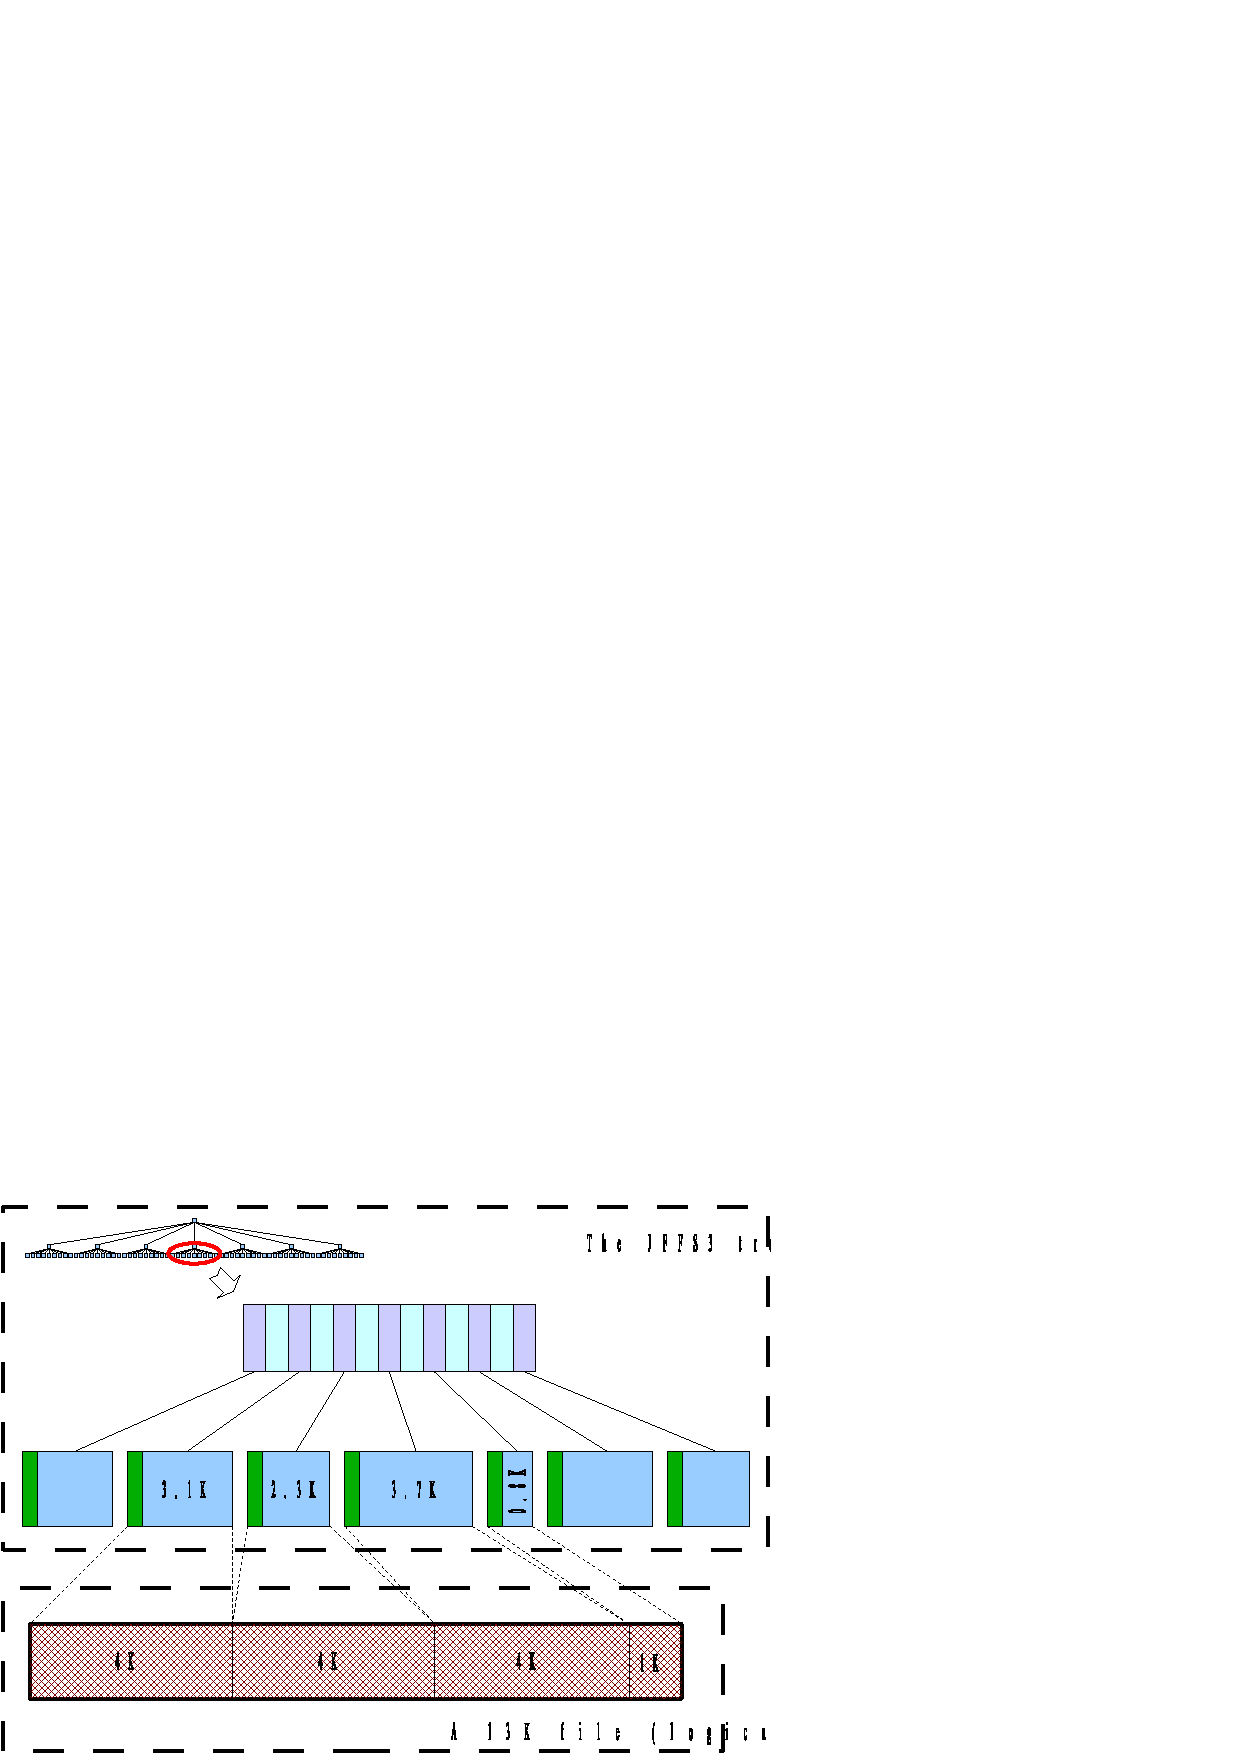
\includegraphics[width=130mm,height=85mm]{pics/dataobj-01.pdf}
%end{latexonly}
\end{center}
\caption{An illustration of files' data representation.}
\label{ref_FigureDataObj-01}
\end{figure}

Figure~\ref{ref_FigureDataObj-01} illustrates the correspondence between files'
contents and data objects. Each \mbox{RAM~page-size} piece of a 13K file
corresponds to a data node in the JFFS3 tree. The 1K tail of the file also
corresponds to a data node. But because of compression actual sizes of data
nodes are less then the corresponding file fragments.

The division on \mbox{RAM~page-sized} fragments relates to the Linux Virtual
Memory Management architecture. Namely, the Linux \emph{Page Cache} works in
terms of RAM pages which means, that JFFS3 is always asked to read and write
files' in units of RAM page size.

It is worth noting that in order to optimize flash utilization, JFFS3 may store
multiple of \mbox{RAM page} bytes in one data node for static files. This
admits of better compression and leads to several other benefits.

\item \emph{Direntry} objects contain the correspondence between directory
entry names and inode numbers. Direntry objects are stored in \emph{direntry
nodes}. Every directory entry in the file system has a corresponding direntry
object.

\item \emph{Attr-data} objects contain attributes of inodes~-- both standard
Unix attributes like user~ID, last modification time, inode
length, etc and \mbox{JFFS3-specific} attributes like the type of compression,
etc. Each inode has only one corresponding \mbox{attr-data} object.

\item \emph{Xentry} objects contain the correspondence between names of
extended attributes and \emph{xattr~IDs}. Every extended attribute in the file
system has a corresponding xattr entry object. This is analogous to direntry
objects, but direntries contain
\{\texttt{direntry~name}$\Rightarrow$\texttt{inode~number}\} mapping, instead
of \{\texttt{xattr~name}$\Rightarrow$\texttt{xattr~ID}\} mapping in xentries.

Each extended attribute in JFFS3 has its own unique number~-- xattr~ID, just
like every inode has its own unique inode number. And in fact, JFFS3 utilizes
the same space of numbers to enumerate inodes and extended attributes. 

Xentry objects are stored in \emph{xentry nodes}.

\item \emph{Xattr-data} objects contain the data of extended attributes. The
way how \mbox{xattr-data} objects are kept in the tree is equivalent to the way
how data objects a kept there. \emph{Xattr-data} objects are stored in
\emph{xattr-data} nodes.

\item \emph{Acl} objects contain Access Control Lists (ACL) of inodes
(information about ACLs may be found out at~[\ref{ref_ACL}]). Acl objects are
stored in \emph{acl nodes}.

In \mbox{real-world} systems a vast number of files have equivalent ACL while
only few files have unique ACL. For the former group of files (or more
strictly~-- inodes) JFFS3 makes use of \emph{shared~acl} objects. This means,
that there is only one acl object instance for all of these inodes. Shared acls
are referred to from \mbox{attr-data} objects of these inodes. If a shared acl
is written to, a new acl object is created (\mbox{copy-on-write} mechanism).
Conversely, for the latter group there is a distinct acl object per each inode.

\end{enumerate}

%
% KEYS
%
\subsection{Keys} \label{ref_SectionKeys}

Each object has its own key and may be quickly looked~up in the tree by its
key. As there are 6 object types in JFFS3, there are also 6 key types:

\begin{enumerate}
\item \emph{data keys}~-- index data objects;
\item \emph{direntry keys}~-- index direntry objects;
\item \emph{attr-data keys}~-- index attr-data objects;
\item \emph{xentry keys}~-- index xentry objects;
\item \emph{xattr-data keys}~-- index xattr-data objects;
\item \emph{acl keys}~-- index acl objects.
\end{enumerate}

%
% Trivial key scheme
%
\subsubsection{Trivial key scheme}

Lets start discussing JFFS3 keys with an example of a simple key layout which
is further referred to as the \emph{trivial key scheme}. All keys in this
scheme have the same \mbox{47-bit} length (see figure~\ref{ref_FigureTrivKey}). 

\begin{itemize}

\item Data keys consist of the \mbox{32-bit} inode number the data belongs to,
the unique \mbox{3-bit} key type identifier, and the \mbox{20-bit} data offset.

\item Direntry keys consist of the \mbox{32-bit} parent directory inode number,
the unique \mbox{3-bit} key type identifier, and the \mbox{20-bit} direntry
name hash value.

\item Attr-data keys consist of the \mbox{32-bit} inode number the attributes
belong to, and the unique \mbox{3-bit} key type identifier.

\item Xentry keys consist of the \mbox{32-bit} inode number the extended
attribute belongs to, the unique \mbox{3-bit} key type identifier, and the
\mbox{20-bit} extended attribute name hash value.

\item Xattr-data keys consist of the \mbox{32-bit} xattr ID, the unique
\mbox{3-bit} key type identifier, and the \mbox{20-bit} extended attribute data
offset.

\item Acl keys consist of the \mbox{32-bit} inode number the acl object belongs
to, and the unique \mbox{3-bit} key type identifier.

\end{itemize}

The following is the list of key type identifiers.

\begin{enumerate}

\item Data keys~-- \texttt{0} (\texttt{000} bin);
\item Direntry keys~-- \texttt{1} (\texttt{001} bin);
\item Attr-data keys~-- \texttt{2} (\texttt{010} bin);
\item Xentry keys~-- \texttt{3} (\texttt{011} bin);
\item Xattr-data keys~-- \texttt{4} (\texttt{100} bin);
\item Acl keys~-- \texttt{4} (\texttt{101} bin);

\end{enumerate}

%
% The trivial key scheme
%
\begin{figure}[h]
\begin{center}
\begin{htmlonly}
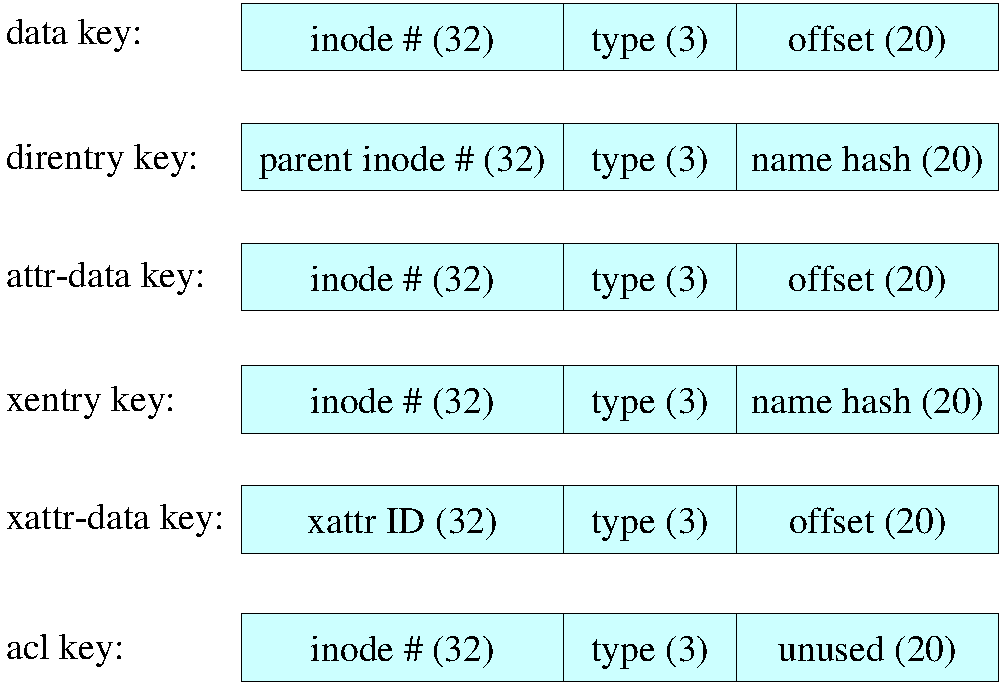
\includegraphics{pics/trivkey-01.png}
\end{htmlonly}
%begin{latexonly}
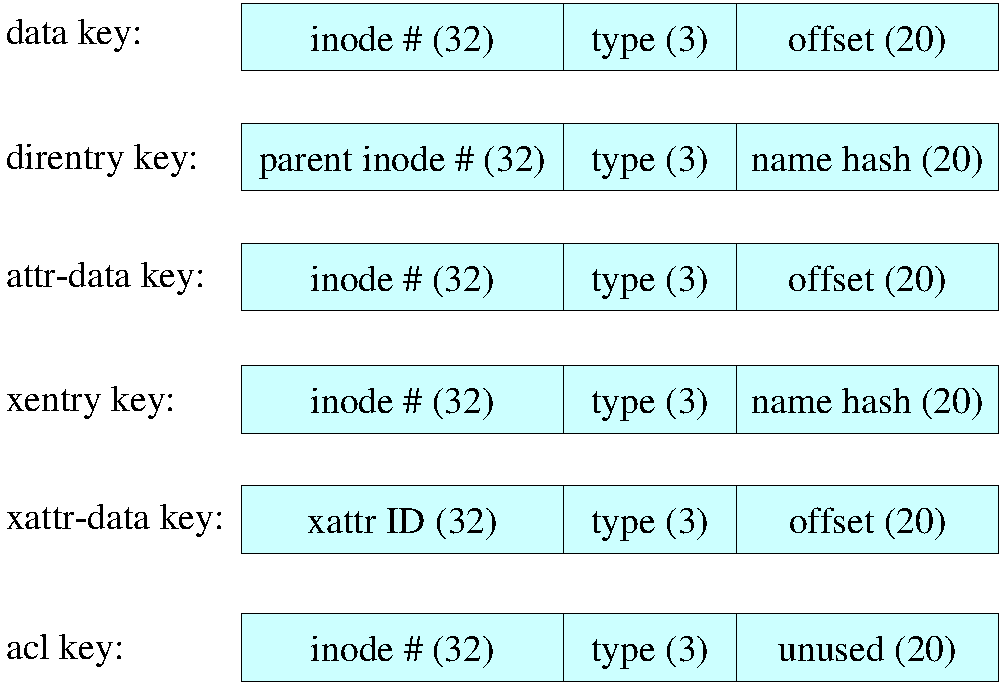
\includegraphics[width=110mm,height=70mm]{pics/trivkey-01.pdf}
%end{latexonly}
\end{center}
\caption{The trivial key scheme.}
\label{ref_FigureTrivKey}
\end{figure}

Since data objects may only contain multiple RAM~pages of data (excluding small
files and files' tails) offsets in keys are always RAM~page
\mbox{size-aligned}. Assuming RAM~page is 4K (12~bits), 20~bits is enough to
refer up to 4GB of data. To put it differently, the trivial key scheme limits
files' length to 4GB providing system's RAM~page size is 4K.

It is also worth noting that several objects of the same type may have the same
key. For example, in case of hash collision, two direntries may have equivalent
keys. In this case objects may be distinguished by means of reading the
corresponding leaf node headers.

%
% Keys comparison
%
\subsubsection{Keys comparison}

The important topic is how keys are compared as it defines the relative order
of objects in the tree and is crucial for searching. Note, it only makes sense
to compare keys of the same type.

JFFS3 keys are usually comprised of one or more fields, i.e., keys $K_1$ and
$K_2$ may be represented as

$$
K_1 = \{k^1_1, k^2_1, ..., k^p_1\},
K_2 = \{k^1_2, k^2_2, ..., k^p_2\},
$$
where $p$ is the number of components in keys of this type.

Keys $K_1$ and $K_2$ are considered to be \emph{equivalent} if and only if all
their fields are equivalent, i.e. $k^i_1 = k^i_2, i = 1, 2, ..., p$.

Keys are compared \mbox{field-by-field} starting from the first field. If on
$i$'th step $k^i_1 > k^i_2$, then $K_1$ is considered to be \emph{greater} then
$K_2$.  Similarly, if on $i$'th step $k^i_1 < k^i_2$, then $K_1$ is considered
to be \emph{less} then $K_2$.

%
% Key schemes
%
\subsubsection{Key schemes}

\emph{Key schemes} define layout of keys for all the 6 object types.
Apparently, it would be too inflexible to hardcode JFFS3 to support only one
fixed key scheme. Indeed, there may be a great deal of reasons why users may
want to use different key schemes in different situations~-- some examples go
bellow.

\begin{itemize}

\item The inode number is encoded by a \mbox{32-bit} integer in the trivial key
scheme which means that about 4~million inodes and extended attributes may
exist on the file system simultaneously. But in some cases this may be
insufficient or, conversely, too much and one may want to use less bits to
encode inode numbers (say, only 24 bits), just for optimization.

\item Similarly, offsets are encoded as \mbox{20-bit} integers in the trivial
key scheme which may be insufficient when huge files (larger then 4G) should be
supported. So one may want to use more bits in certain cases.

\item Depending on the concrete JFFS3 usage, different hash functions may be
used in direntry keys. The length of hash values may also vary depending on how
many directory entries are kept in directories. If there are huge directories
with millions of files there, long hash values should be used to avoid massive
hash collisions (say, \mbox{64-bit} hash values). But if it is known in advance
that there will be no too large directory entries, \footnote{Note, when talking
about directories, words "\emph{large}" and "\emph{small}" describe how many
direntries are kept in these directories. The more direntries a directory
contains, the larger is it.} the length of hash values may be shorter.

\item It also possible that one may want to use some tricky key layouts to
achieve different kinds of optimization. For example, direntry keys may
include the first 8~bytes (64~bits) of the direntry name (see figure
\ref{ref_FigureDirentKeyEx_01}). In this case the \texttt{getdents}
\footnote{See \texttt{getdents (2)} Linux manual pages} Linux system call will
return direntries in "mostly" alphabetically sorted order and \mbox{user-space}
programs will not spend much time to sort them. In fact this technique is used
in the Reiser4 file system and it is claimed that slow sorting is a bottleneck
in certain \mbox{real-life} workloads. And the like.

\item Different keys compression methods may be used in different key schemes
(see section \ref{ref_SectionKeysCompr} below).

\end{itemize}

%
% Direntry key layout example
%
\begin{figure}[h]
\begin{center}
\begin{htmlonly}
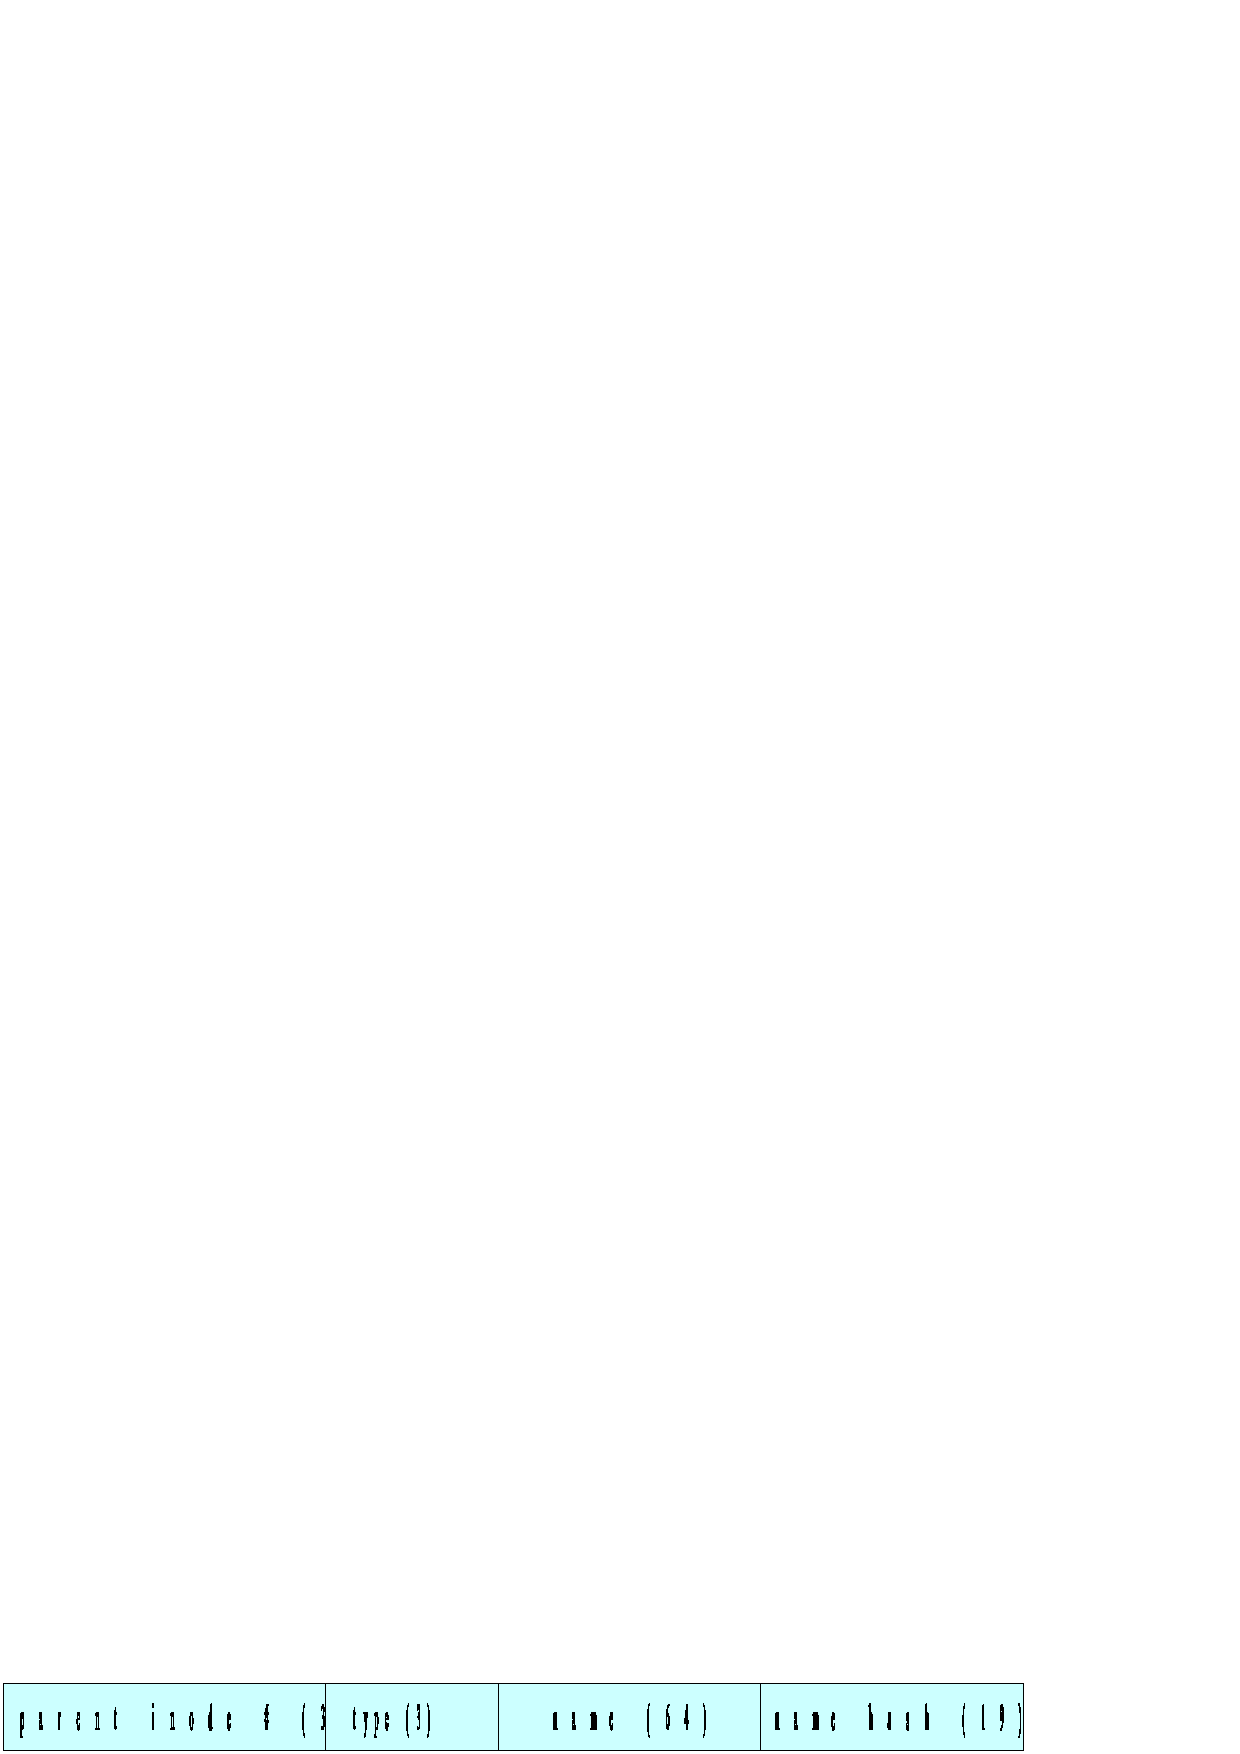
\includegraphics{pics/keyex-01.png}
\end{htmlonly}
%begin{latexonly}
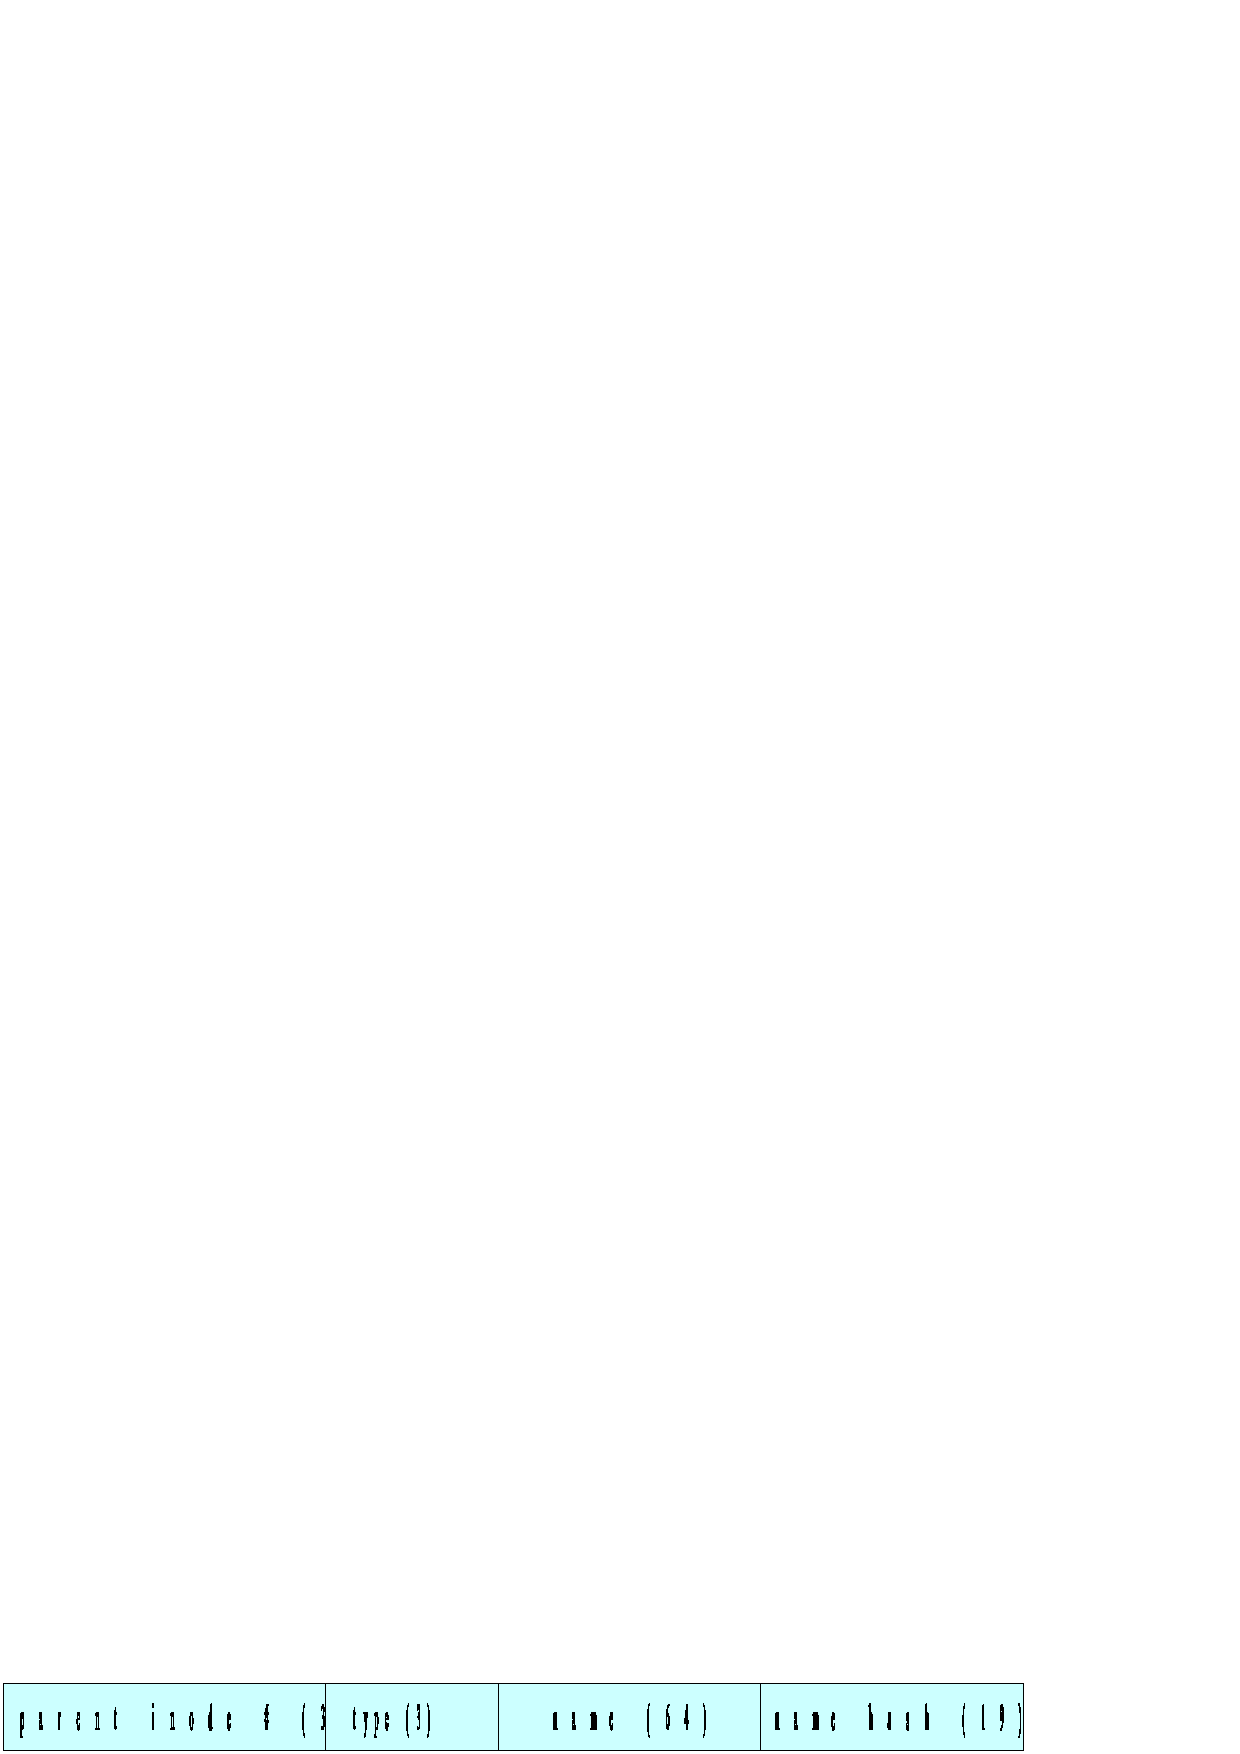
\includegraphics[width=110mm,height=7mm]{pics/keyex-01.pdf}
%end{latexonly}
\end{center}
\caption{Direntry key layout example.}
\label{ref_FigureDirentKeyEx_01}
\end{figure}

So it is obvious why JFFS3 is not attached to a fixed key scheme but instead,
admits of many different key schemes (one at a time of course) with a
possibility to choose the best suited key scheme.

%
% Keys compression
%
\subsubsection{Keys compression} \label{ref_SectionKeysCompr}

The index is the most frequently \mbox{re-written} part of JFFS3. Indeed, every
single change at the leaf level of the tree requires \mbox{re-writing} $L-1$
indexing nodes. The number of index updates is reduced by the
\mbox{write-behind} cache and by the \mbox{journal}, but it is still changed
very often.  So, it is extremely important for JFFS3 to keep the tree as
shallow as it is possible.

This means, that it makes sense to apply a sort of compression to keys in
indexing nodes. There are several ways to compress keys and the following are
examples of possible compression techniques.

\begin{description}

\item[Offsets coding.] Offsets compression may be based on the observation that
the overwhelming majority of files in many file systems are small files. This
means, that it might makes sense to code smaller offsets by fewer bits.

Table \ref{ref_TableOffsCodes} contains an example of how offsets may be
encoded. For offsets in range \texttt{0KB-8KB} only 3~bits are enough, so the
bit sequence "\texttt{000}" will encode offset \texttt{0}, and the bit sequence
"\texttt{001}" will encode offset \texttt{4K} \footnote{Recall, offsets in keys
are \mbox{RAM page-aligned} and by default, the RAM~page size is assumed to be
4K in this document}. Offsets in range \texttt{8KB-64KB} are encoded by 6~bits
and so on.

\begin{table}[h]
\begin{center}
\begin{tabular}{llll}
\textbf{Offset range} & \textbf{Bits in range} & \textbf{Code prefix} & \textbf{Code length}\\
\hline
\texttt{0KB-8KB}   & 13 bits & \texttt{00}  & 3 bits\\
\texttt{8KB-64KB}  & 16 bits & \texttt{01}  & 6 bits\\
\texttt{64KB-1MB}  & 20 bits & \texttt{10}  & 10 bits\\
\texttt{1MB-128MB} & 27 bits & \texttt{110} & 18 bits\\
\texttt{128MB-4GB} & 32 bits & \texttt{111} & 23 bits\\
\end{tabular}
\caption{An example of offset coding.}
\label{ref_TableOffsCodes}
\end{center}
\end{table}

\item[Inode number coding.] If the approximate number of inodes on the
file system is known in advance, similar coding scheme may be exploited for
inode numbers providing JFFS3 may reuse deleted files' inode numbers.

\item[Common prefix compression.] In case of the trivial key scheme the first
field of any key is the inode number. Any other key scheme will likely also
contain the inode number in keys. If the inode number is the first component of
the key, all keys belonging to the same inode will go sequentially in indexing
nodes. To put it differently, there will be sequences of keys prefixed by the
same inode number in the tree.

%
% Common prefix compression example
%
\begin{figure}[h]
\begin{center}
\begin{htmlonly}
\includegraphics{pics/comprex-01.png}
\end{htmlonly}
%begin{latexonly}
\includegraphics[width=160mm,height=40mm]{pics/comprex-01.pdf}
%end{latexonly}
\end{center}
\caption{The common prefix compression idea illustration.}
\label{ref_FigureKeyComprEx_01}
\end{figure}

The evident compression method for these key sequences is to store the inode
number only once as the common prefix for the entire key sequence, instead of
duplicating it in every key. Figure \ref{ref_FigureKeyComprEx_01} illustrates
how does the prefix compression work.

\item[Offsets sequence compression.] In the trivial key scheme the last field
of data keys is the offset. The offset is multiple of RAM~page size. Obviously,
indexing nodes will contain sequences of keys each of which describes data
objects belonging to the same file but with different offsets. Moreover, the
keys will be ordered in increasing key order. 

For sequences like this it is possible to only specify the starting offset, the
ending offset and the number of keys in the sequence, instead of wasting space
storing the offset in each key of the sequence.

%
% Offsets sequence compression example
%
\begin{figure}[h]
\begin{center}
\begin{htmlonly}
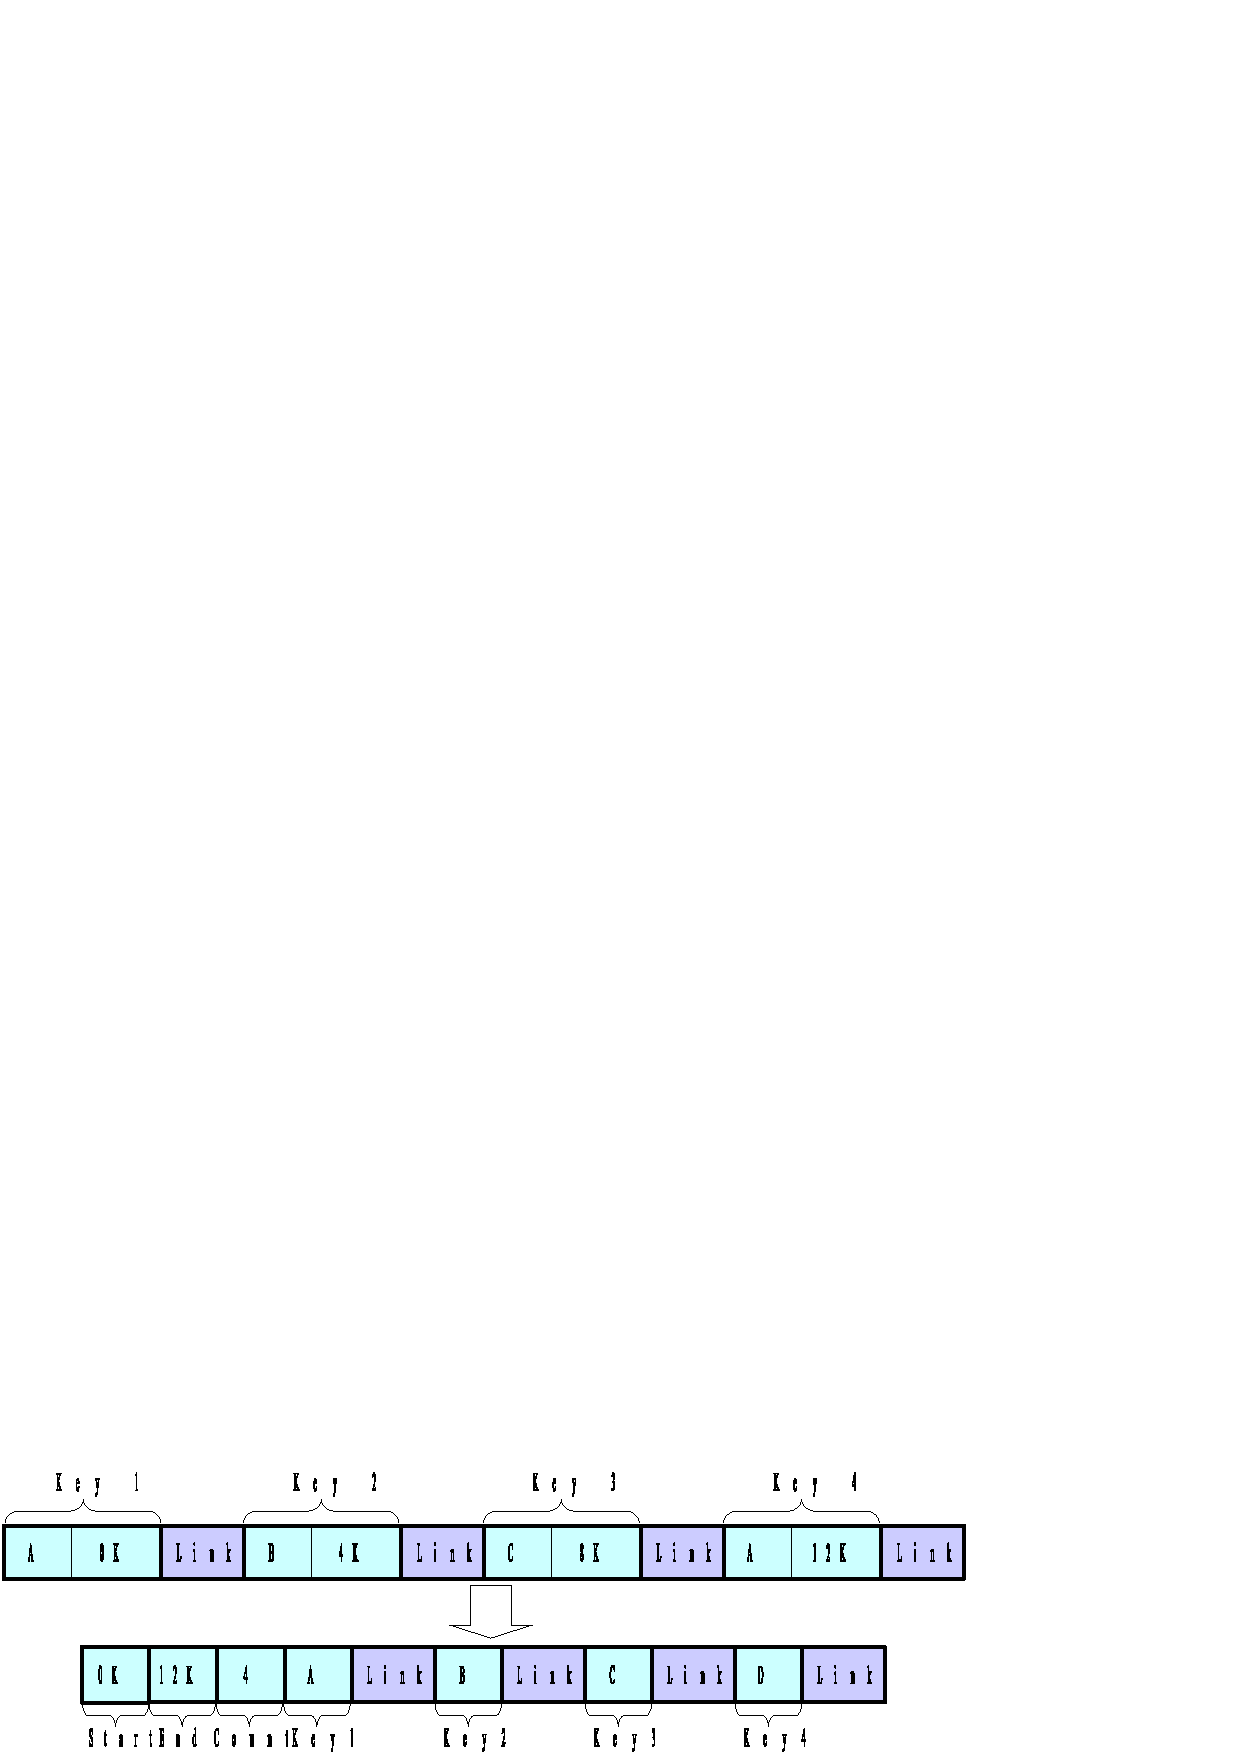
\includegraphics{pics/comprex-02.png}
\end{htmlonly}
%begin{latexonly}
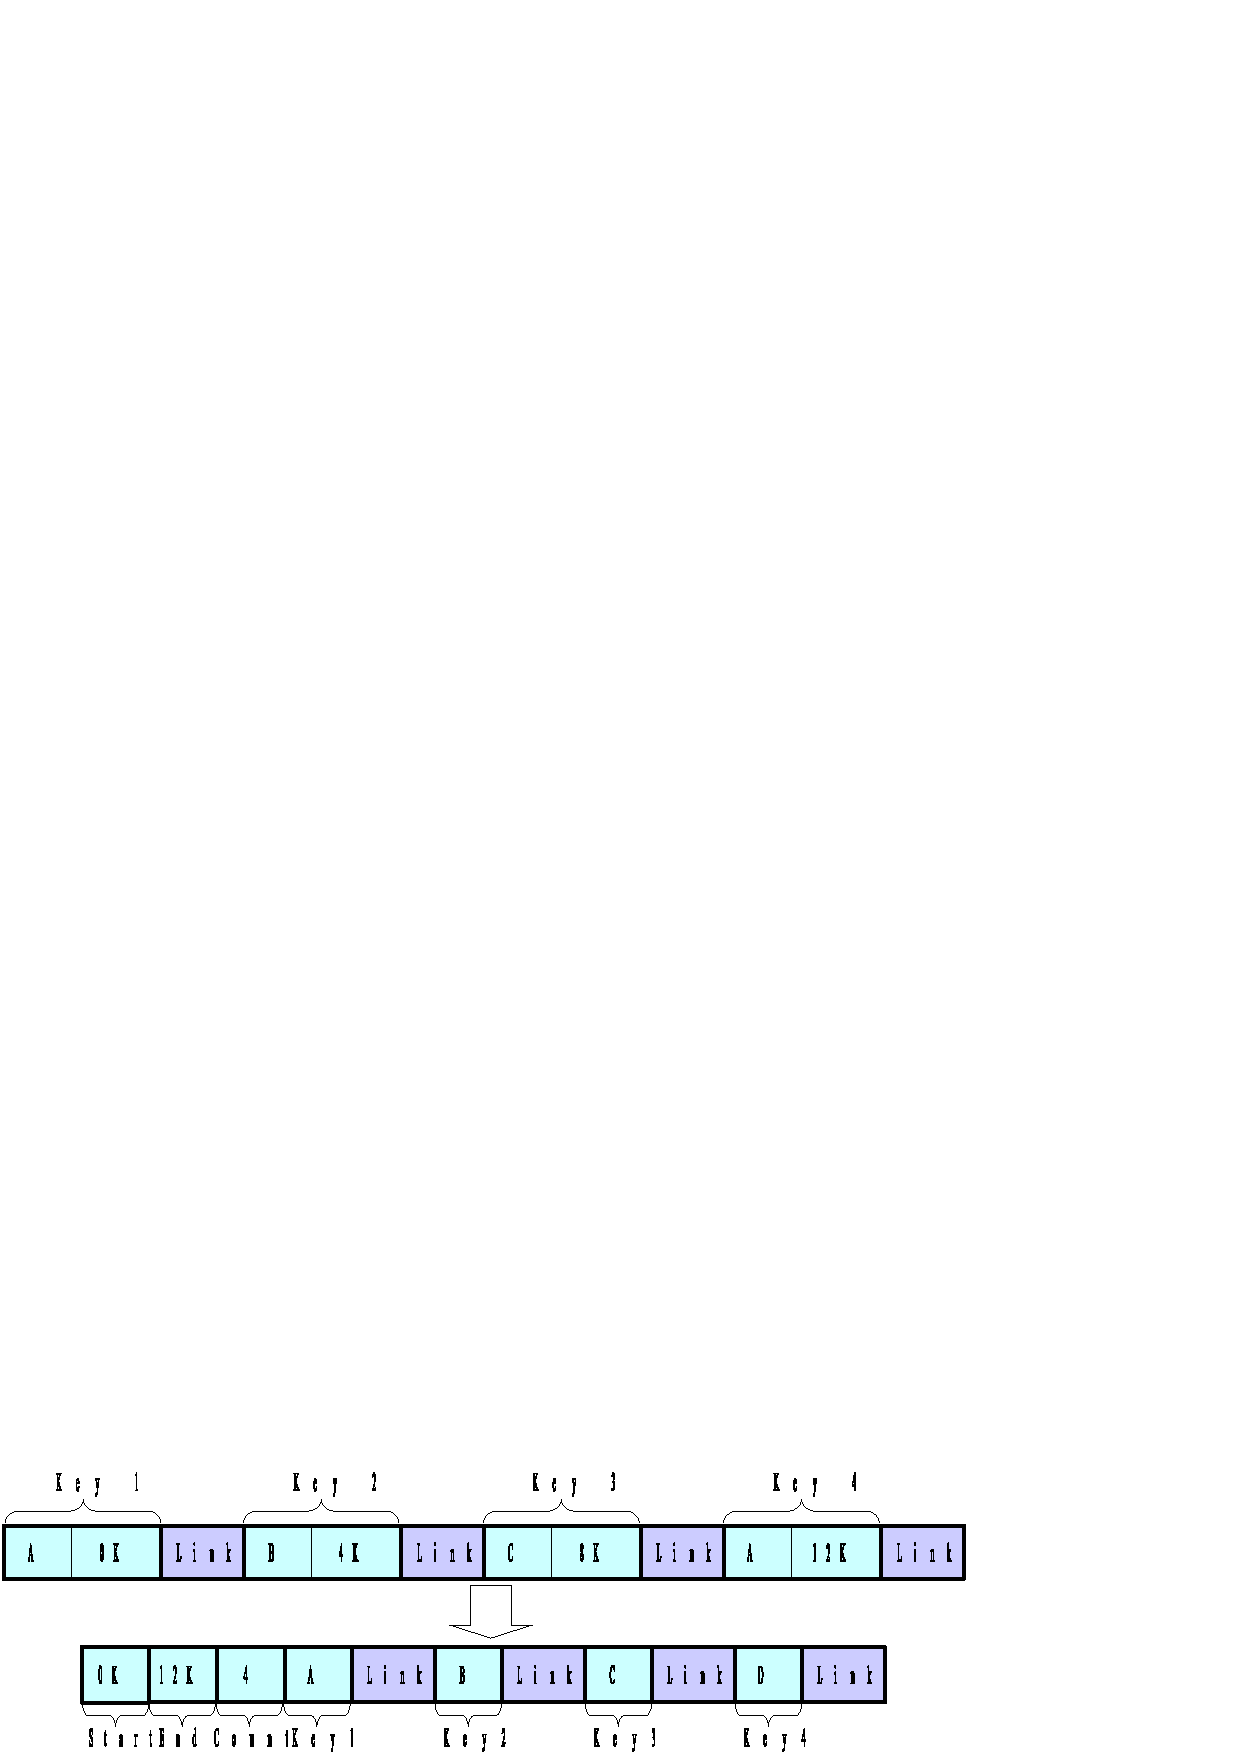
\includegraphics[width=160mm,height=42mm]{pics/comprex-02.pdf}
%end{latexonly}
\end{center}
\caption{The Offsets sequence compression idea illustration.}
\label{ref_FigureKeyComprEx_02}
\end{figure}

Figure \ref{ref_FigureKeyComprEx_02} presents an example of the offsets sequence
compression method. Four consecutive keys which describe four data objects
belonging to the same inode may be represented as a sequence of four keys
without the offset field, but prefixed by the starting offset, the ending
offset and the number of keys in the sequence.

\end{description}

Note, the above compression methods may be combined to achieve better
compression.

Because of compression, JFFS3 keys have variable size which means, that it is
impossible to directly apply the binary search algorithm to the contents of
indexing nodes. In JFFS3, indexing nodes are decompressed when read and are
cached in decompressed form. And after the indexing node has been decompressed,
the binary search algorithm is applicable.

We believe that keys compression will considerably reduce the amount of
\mbox{on-flash} indexing information and increase the overall performance just
because the amount of Input/Output will lessen. But only actual
\mbox{fixed-size} keys~vs.~\mbox{variable-size} keys tests will show if there
is some real performance gain present.

%
% LINKS
%
\subsection{Links} \label{ref_SectionKeys}

Links in JFFS3 have fixed length and are not compressed. The link width depends
on the size of JFFS3 partition~-- the larger is JFFS3 partition, the wider are
links. Instead of choosing a huge link width to suit the largest possible file
systems (e.g. 64~bits), JFFS3 admits of flexible links width, depending on
JFFS3 partition size.

As indexind nodes have fixed size equivalent to one sector, the width of links
stored in branch nodes and in the root nodes is

$$
w = log_2{S} - s.
$$
Twig nodes refer variable-size leaf nodes so the width of links stored twih
nodes is
$$
w = log_2{S},
$$
where $S$ is the size of the JFFS3 partition and $s$ is the size of sector.

